\documentclass[]{finalproject}
\usepackage{float}
\usepackage{graphicx}
\usepackage{minted}
\usepackage{ragged2e}
\graphicspath{{./img}}

\captionsetup{labelfont={bf}}

% Title (and subtitle) of the project
\title{Quicksort}
\subtitle{}

% Group members for the final project (comment out the unnecessary entries)
\begin{groupmembers}
\studentA{Pratyai}{}{Mazumder}
\studentB{Lodovico}{}{Mazzei}
\studentC{Michele}{}{Chersich}
\end{groupmembers}

\abstract {
A short abstract summarising what your project is about and the main results you obtained.
}


\begin{document}
\maketitle

\section{Introduction} \label{introduction}
\subsection{The sorting problem}

\section{The algorithm}
\subsection{The partitioning problem}

\section{Complexity analysis}
\subsection{Worst-case analysis}
\subsection{Average-case analysis}
\subsection{Analysis of randomized Quicksort}

\section{Parallel processing}
\subsection{Scaling features}
\subsection{Parallelizing Quicksort}

\section{Computational geometry and the convex hull problem}
Computational geometry is the study of algorithms for the solution of geometric problems in the Euclidean space \cite{paper}.
The convex hull problem belongs to this class of problems. It is defined as follows:
given a set of points, find the smallest convex polygon containing all the points \cite{geowiki}.
The problem has wide range of applications in
mathematics, statistics, combinatorial optimization, economics, geometric modeling, and ethology \cite{chwiki}.
For the purpose of this project, we will consider only the planar convex hull (i.e. 2D Euclidean space).

\subsection{The Quickhull algorithm}
The Quickhull algorithm applies the algorithm design principles of Quicksort to the solution of the convex hull problem.
The algorithms works as follows:
the set of points is split into smaller subproblems by partitioning.
The first partitioning step is done by picking the two points with minimum and maximum x-coordinates:
the line connecting these points splits the set into two subdomains.
Then, we apply a recursive procedure on both subdomains.
First, we search for the point that is farthest away from the line.
If no point is found, then there is no points lying outside the line, so we can add the two points to the convex hull.
Otherwise, we partition the subset again with the two lines, joining the newfound point and each of the two points, respectively.
Then, we apply the recursive step again, searching for the solution only in the subsets of points that lie outside the two lines.
The very first steps of the algorithm are illustrated in Figure \ref{fig:qh-steps}.

\begin{figure}[H]
    \centering
    \begin{minipage}{.33\linewidth}
		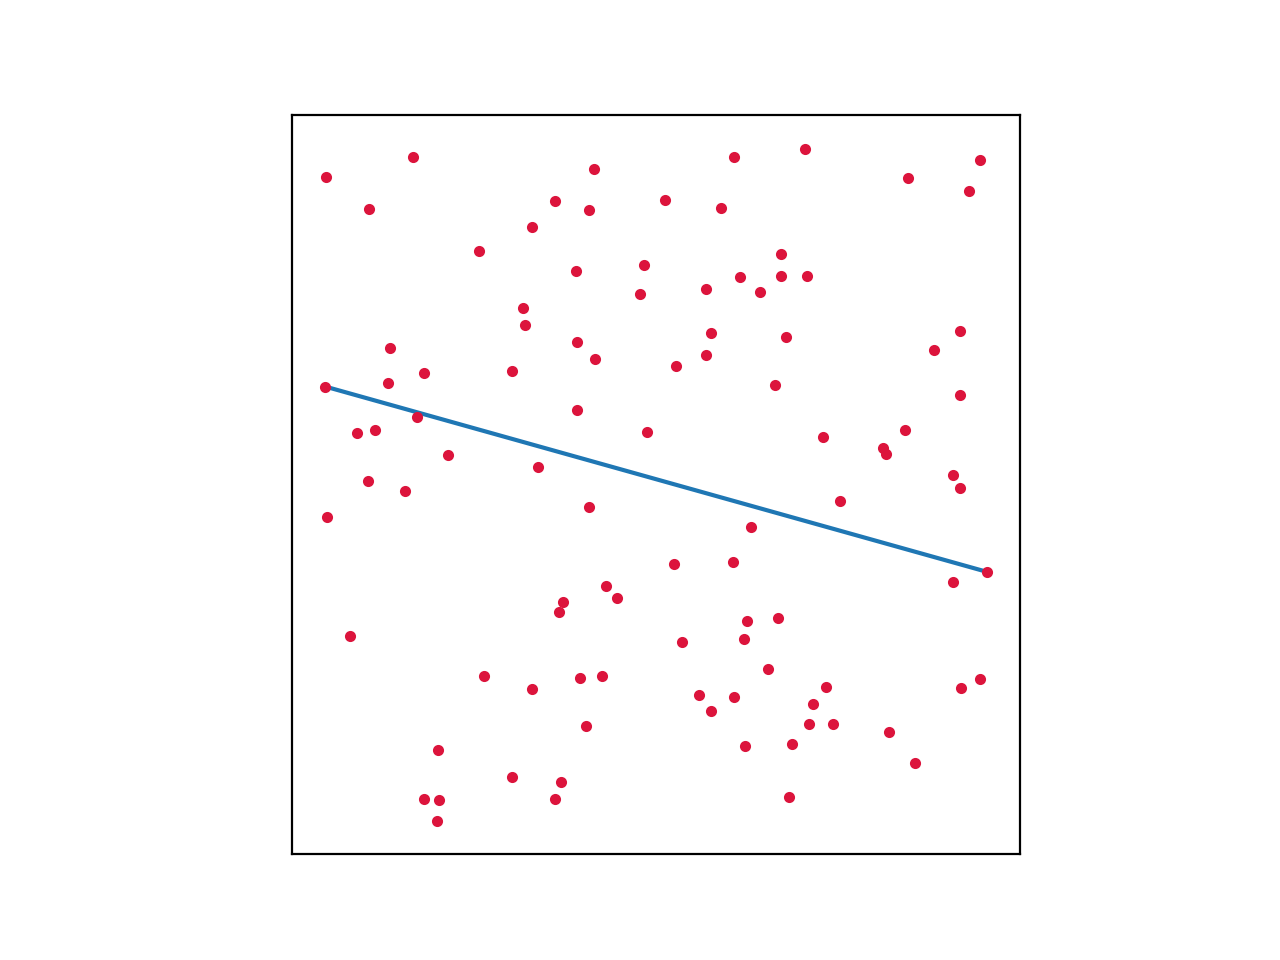
\includegraphics[width=\linewidth]{quickhull1.png}
	\end{minipage}
	\begin{minipage}{.33\linewidth}
		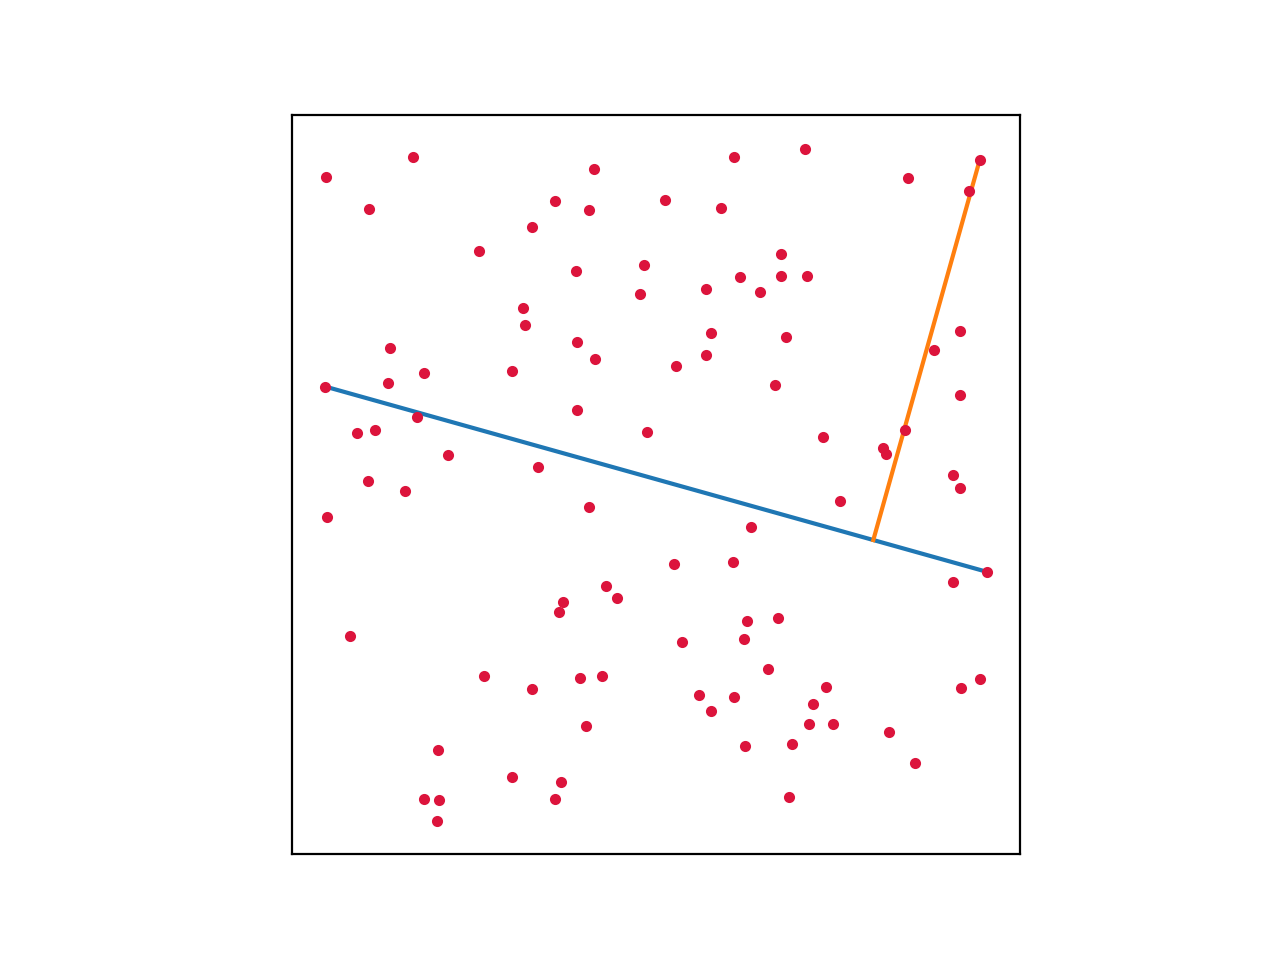
\includegraphics[width=\linewidth]{quickhull2.png}
	\end{minipage}
    \begin{minipage}{.33\linewidth}
		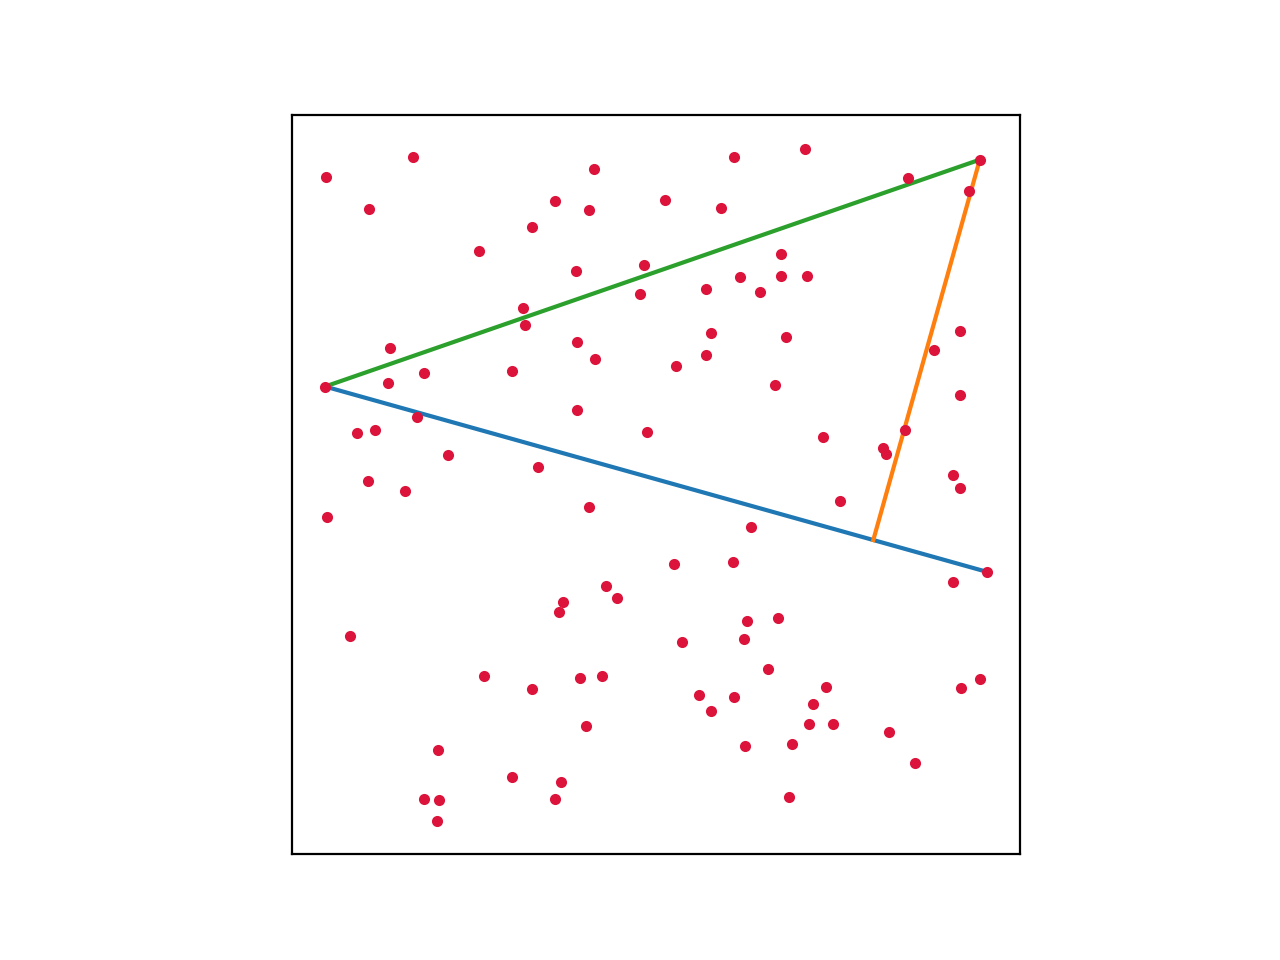
\includegraphics[width=\linewidth]{quickhull3.png}
	\end{minipage}
    \caption{The set of points is partitioned in two subsets (left); the farthest point from the line is found (middle); the triangle's hypotenuse identifies either two points in the solution set, or an outer subset of points, in which part of the solution can be found (right).}
    \label{fig:qh-steps}
\end{figure}

The pseudocode of the algorithm is given below:
\begin{verbatim}
    pseudocode goes here
\end{verbatim}

\raggedright We can observe similarities between Quicksort and Quickhull,
as both are divide-and-conquer and sorting algorithms. The former principle is applied by partitioning the domain
and splitting the initial problem into smaller subproblems, whereas the latter is applied by comparing
Euclidean distances of points.


\subsection{Distributed Quickhull}
The Quickhull algorithm is sequential by design,
as each recursive call depends on the previous ones for the computation of the solution set \cite{qhpaper}.
Therefore, parallelizing the algorithm by multithreading is not feasible.
Also, although the recursive step allows to discriminate among subsets of points to compute the solution,
the selection is done by computing Euclidean distances. Therefore, the size of the point set does not decrease
in the recursive step and execution gets significantly slow for large input sets.
However, the set of points can be distributed over multiple processes, and the algorithm does scale by multiprocessing.\\
The pseudocode of the distributed version of the algorithm is given below:
\begin{verbatim}
    parallel pseudocode goes here
\end{verbatim}

\raggedright As we can see, the procedure is almost identical to the sequential version.
The key difference is the addition of collective communication (\verb|allreduce|) among processes in the partitioning steps:
the computation performed by each process to find the first two partitioning points, as well as the farthest point at every iteration,
is limited to a subset of points, so the results from each process must be combined, in order to obtain the global result.\\
Running the algorithm for large input sizes with different numbers of processes, we can observe significant gains in performance.
A scaling chart is reported in Figure \ref{fig:qh-scaling}.

\begin{figure}[H]
    \centering
    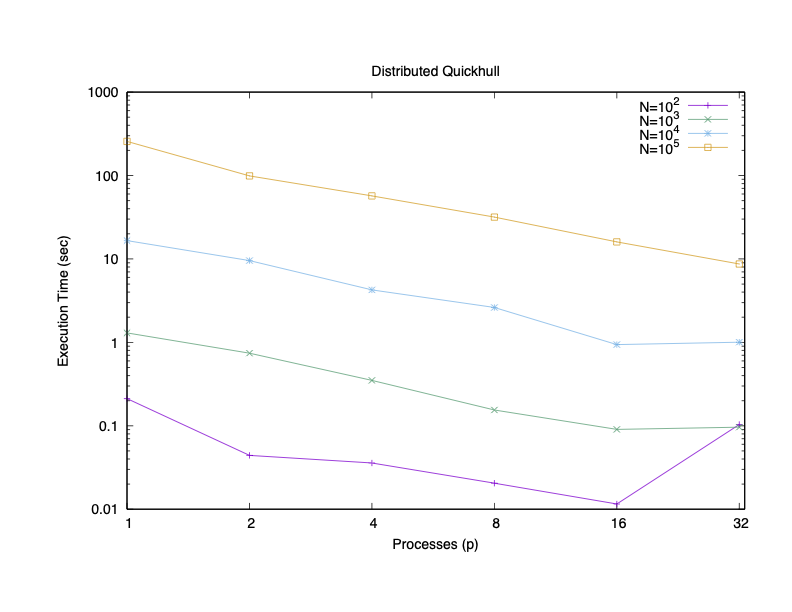
\includegraphics[width=0.7\linewidth]{gpStrongTime.png}
    \caption{Scaling of distributed Quickhull.}
    \label{fig:qh-scaling}
\end{figure}

We can observe the gain in performance obtained by the parallel version of the algorithm:
by doubling the number of processes, the execution time roughly halves.
However, we can also observe the effect of over-parallelizing with respect to the problem size:
for $N=10^2$, 32 processes performe worse than 16.

%%%%%
\clearpage
\bibliographystyle{abbrv}
\bibliography{references}



\end{document}